\chapter{Results and Performance}
%
The generation of the data from the calibrated time series, i.e. the direct
detector response on air-shower photons, is what differs the PhotonStream data
from previous data representations. By finding single photons the goal is to
neglect the noise that is intrinsic when integrating over time series and
getting a more accurat time information. However, the results of this procedure
yield a different data set, so it is important to investigate the differences.

\section{Photon Extraction}
%
The Photon Extraction is the key difference when generating PhotonStream data.
It does not calculate the photon features from the time series but aims at
finding the single photon pulses, which opens the possibility of generating
arrival times per photon and hopefully yields an acurate description of the
air-showers. When comparing the PhotonStream data to the standard data
representation, the intuitive questions at hand are:
%
\begin{enumerate}
  \item What is the difference concerning the number of reconstructed photons?
  \item What is the difference in the number of noise photons?
  \item What is the difference between simulations and data?
\end{enumerate}
%
\begin{figure}
  \begin{subfigure}{\textwidth}
    \centering
    \includegraphics[width=1.2\textwidth, page=17]{Plots/pe_difference_pe_20131104_162.pdf}
  \end{subfigure}
  \begin{subfigure}{\textwidth}
    \centering
    \includegraphics[width=1.2\textwidth, page=26]{Plots/pe_difference_pe_20131104_162.pdf}
  \end{subfigure}
  \begin{subfigure}{\textwidth}
    \centering
    \includegraphics[width=1.2\textwidth, page=33]{Plots/pe_difference_pe_20131104_162.pdf}
  \end{subfigure}
  \begin{subfigure}{\textwidth}
    \centering
    \includegraphics[width=1.2\textwidth, page=53]{Plots/pe_difference_pe_20131104_162.pdf}
  \end{subfigure}
  \caption{PE differences between PhotonStream and Standard.}
  \label{fig:difference}
\end{figure}

%
\begin{figure}
  \begin{subfigure}{0.5\textwidth}
    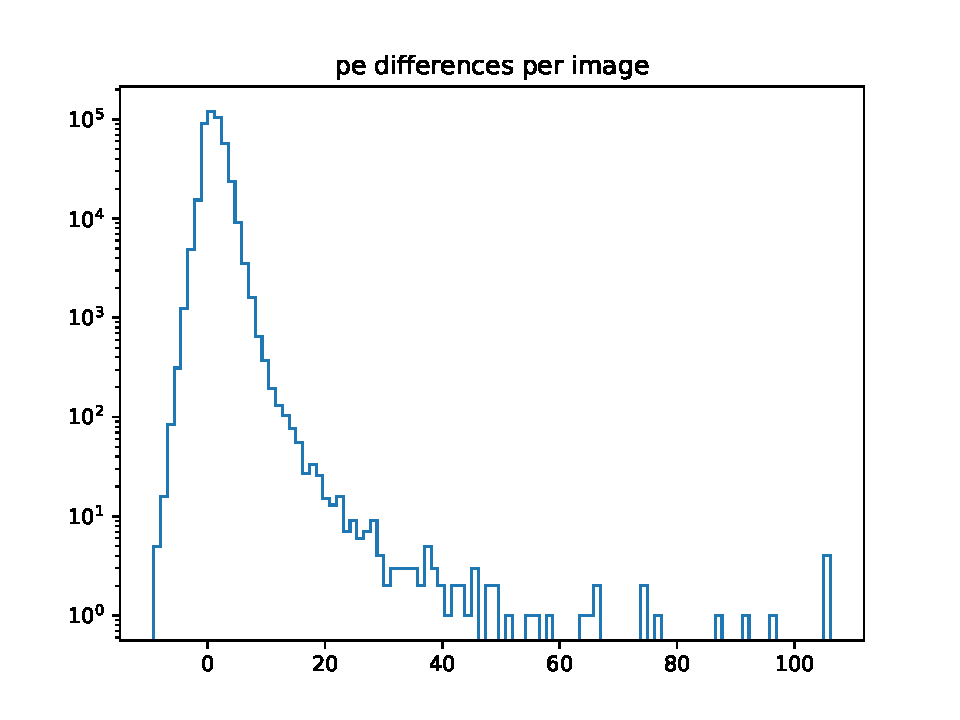
\includegraphics[width=1.1\textwidth]{Plots/diffs_hist_DBSCAN_pe_20131104_162_logy.pdf}
  \end{subfigure}
  \begin{subfigure}{0.5\textwidth}
    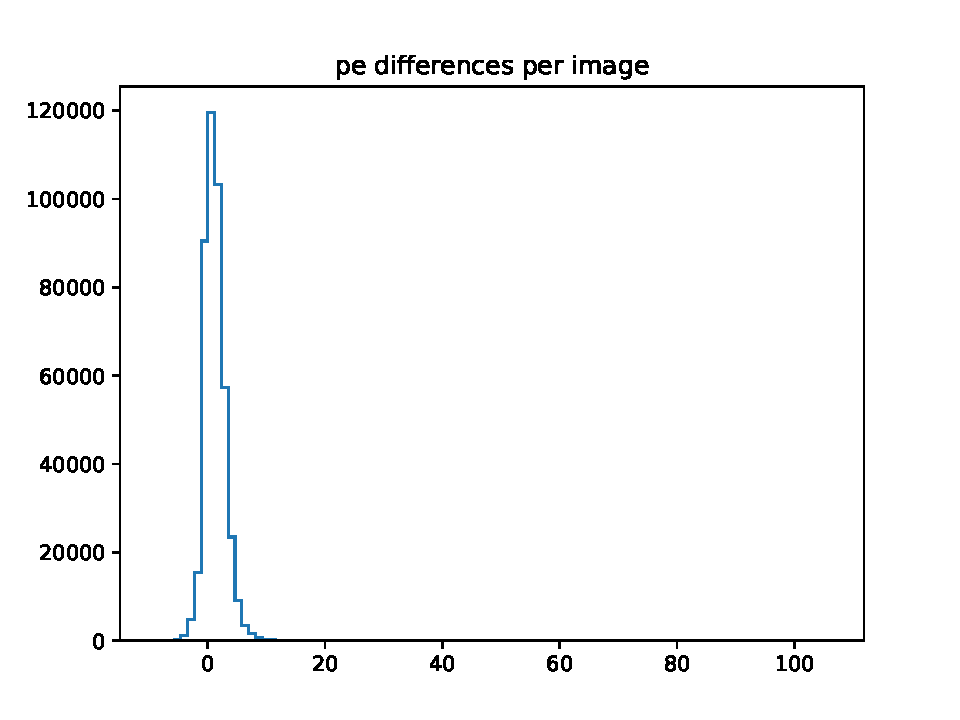
\includegraphics[width=1.1\textwidth]{Plots/diffs_hist_DBSCAN_pe_20131104_162.pdf}
  \end{subfigure}
  \caption{PE differences between Standard and PhotonStream.}
  \label{fig:pe_diffs}
\end{figure}


\section{Time features of PhotonStream?}
%
\begin{figure}
  \begin{subfigure}{0.5\textwidth}
    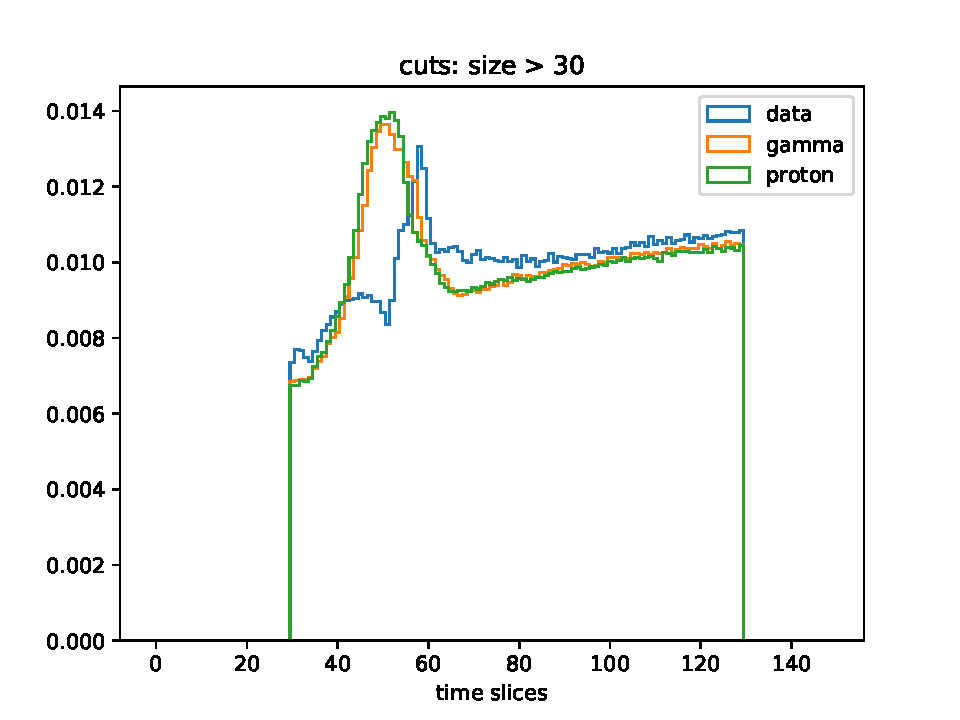
\includegraphics[width=1.1\textwidth]{Plots/all_slices.pdf}
  \end{subfigure}
  \begin{subfigure}{0.5\textwidth}
    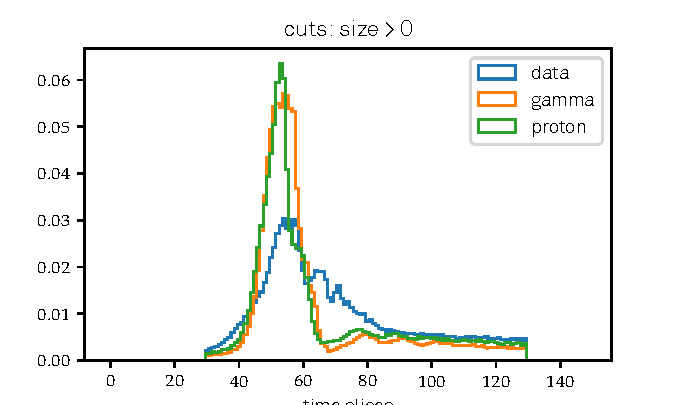
\includegraphics[width=1.1\textwidth]{Plots/all_slices_10_per_pixel.pdf}
  \end{subfigure}
  \caption{Caption.}
  \label{fig:slices}
\end{figure}

\section{Features on the PhotonStream}
%


\section{Origin Reconstruction}
%
\begin{figure}
  \begin{subfigure}{0.5\textwidth}
    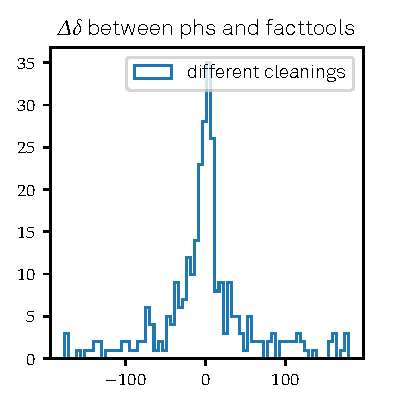
\includegraphics[width=1.1\textwidth]{Plots/delta_diff_hist_DBSCAN_pe_20131104_162.pdf}
  \end{subfigure}
  \begin{subfigure}{0.5\textwidth}
    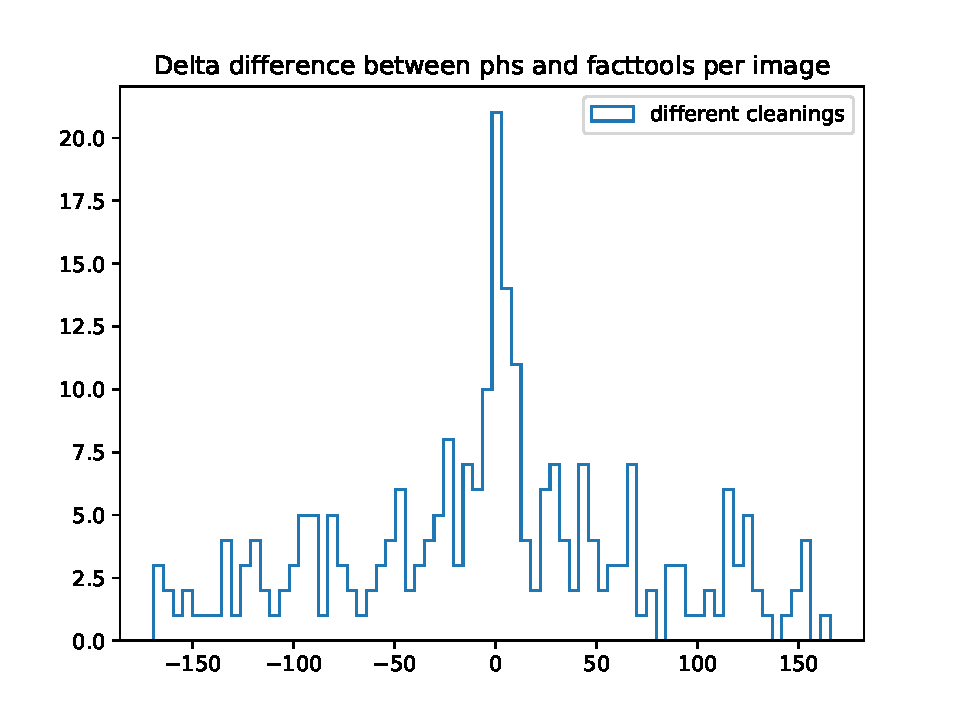
\includegraphics[width=1.1\textwidth]{Plots/delta_diff_hist_thresholds_pe_20131104_162.pdf}
  \end{subfigure}
  \begin{subfigure}{0.5\textwidth}
    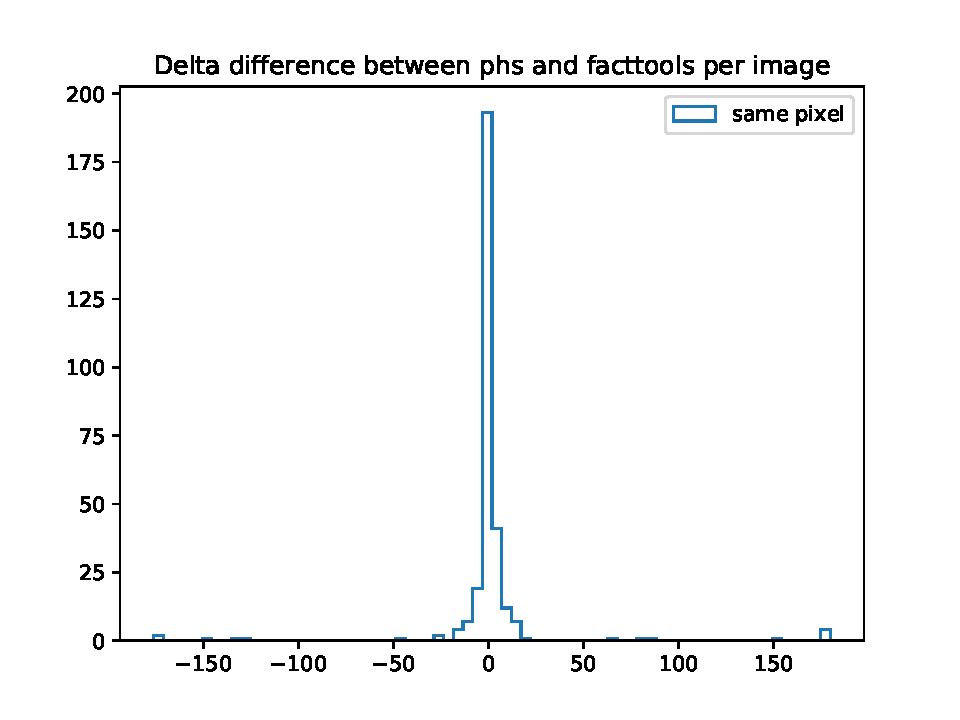
\includegraphics[width=1.1\textwidth]{Plots/delta_hist_same_cleaning_pe_20131104_162.pdf}
  \end{subfigure}
  \begin{subfigure}{0.5\textwidth}
    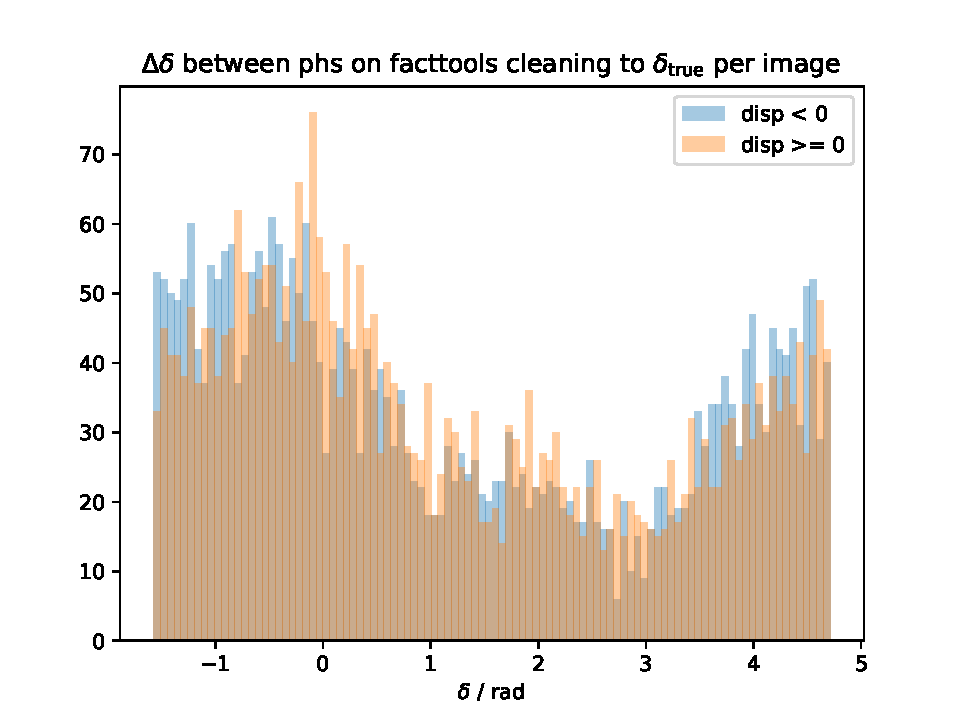
\includegraphics[width=1.1\textwidth]{Plots/delta_true_diff_hist_thresholds_rad_20131104_162.pdf}
  \end{subfigure}
  \caption{Caption.}
  \label{fig:delta}
\end{figure}

\section{Evaluation of the image cleaning}
%
\section{Parameters of DBSCAN}
%
\begin{figure}
  \centering
  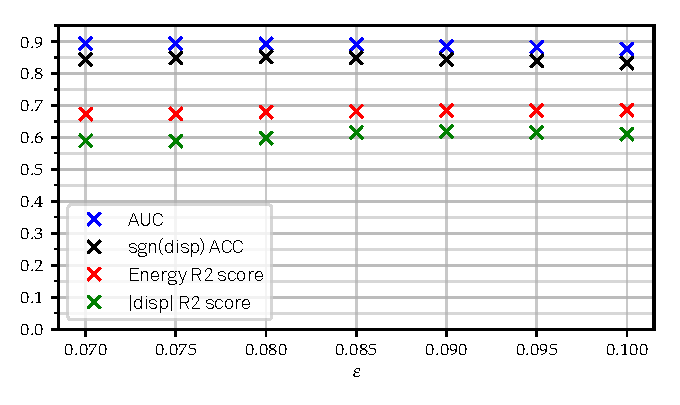
\includegraphics[width=0.7\textwidth]{Plots/Epsilon/eps_scores.pdf}
  \caption{Scores.}
  \label{fig:eps_scores}
\end{figure}
%
\begin{figure}
  \centering
  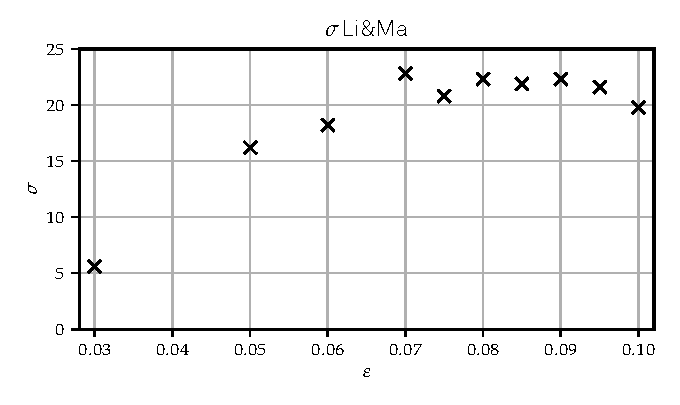
\includegraphics[width=0.7\textwidth]{Plots/Epsilon/eps_sigma.pdf}
  \caption{Detection significance.}
  \label{fig:eps_sigma}
\end{figure}
%
\begin{figure}
  \centering
  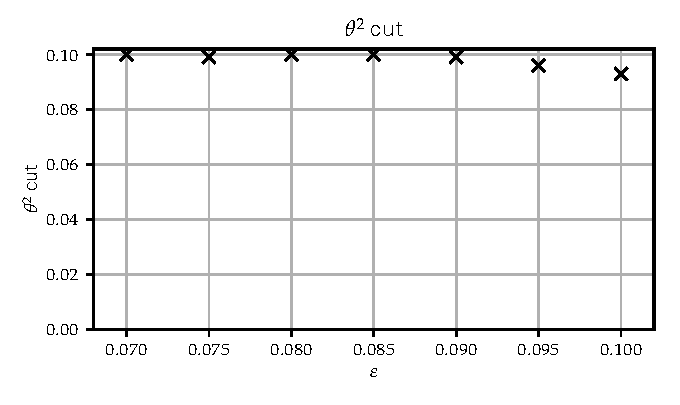
\includegraphics[width=0.7\textwidth]{Plots/Epsilon/eps_theta_cut.pdf}
  \caption{Detection $\theta^2$ cuts.}
  \label{fig:eps_theta}
\end{figure}

\section{Pixelbased Threshold Cleaning on the PhotonStream}
%
